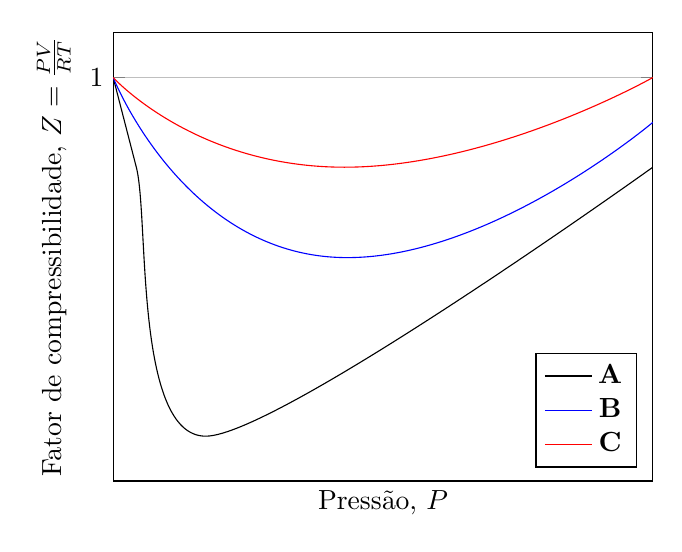
\begin{tikzpicture}
    \begin{axis}
        [
            grid = major,
            legend pos = south east,
            xlabel = {Pressão, $P$},
            ylabel = {Fator de compressibilidade, $Z = \frac{PV}{RT}$},
            xtick=\empty, 
            ytick= 1,
            xmin=0, ymin=0.1,
            xmax=7, ymax=1.1,
        ]
    \addplot[smooth] coordinates
        {
            (0, 1)
            (0.3, 0.8)
            (1.2, 0.2)
            (7, 0.8)
        };
    \addplot[smooth, tension=1, blue] coordinates
        {
            (0, 1)
            (2.8, 0.6)
            (7, 0.9)
        };
    \addplot[smooth, tension=1, red] coordinates
        {
            (0, 1)
            (3, 0.8)
            (7, 1)
        };
    \legend{\textbf{A},\textbf{B},\textbf{C}}
\end{axis}
\end{tikzpicture}